V priponskem drevesu nad besedo $T$ dolžine $n$ na vsako vozlišče, razen na koren, kaže ena povezavo, ki in priponska. To lahko vidimo na zgornjem delu Slike \ref{fig:SuffuxArray}, na katerem je prikazano priponsko drevo za besedo \enquote{KOKOŠ$\$$}, da v vsako vozlišče kaže črna puščica. Vsako vozlišče razen korena ima tudi povezavo na svojega starša. Na Sliki \ref{fig:SuffuxArray} teh povezan ni prikazanih. Vsako notranje vozlišče v priponskem drevesu pa vsebuje tudi priponsko povezavo in le te so na Sliki \ref{fig:SuffuxArray} prikazane s sivo črtkano puščico. Priponsko drevo ima $n$ listov in $n_v$ notranjih vozlišč, zato potrebuje $2(n_v-1+n)+n_v= 3n_v-2+2n$ povezav. Priponsko drevo ima največ $n-1$ notranje vozlišče, torej priponsko drevo potrebuje med $2n+1$ in $5n -5$ povezav.

\begin{figure}[htb]
    \begin{subfigure}[t]{\linewidth}
        
        \includesvg[scale=.8]{Slike/KOKOŠMcCreightS1.svg}
        \centering
        \subcaption*{}
        \label{fig:bSADrevo}
    \end{subfigure}
    \begin{subfigure}[t]{1\linewidth}        
        \includesvg[scale=1.2]{Slike/KokosSA.svg}
        \centering
        \subcaption*{}
        \label{fig:bSAPolje}
    \end{subfigure}
    \caption{Primer priponskega drevesa in priponskega polja z dodatnim $LCP$ poljem nad besedo \enquote{KOKOŠ\$}.} 
    \label{fig:SuffuxArray}
\end{figure}

Vsaka povezava iz vozlišča $v_1$ v $v_2$, pri čemer je $\Stars{v_2}=v_1$, predstavlja neprazen podniz besede $T$ in sicer podniz $\alpha$, ki je definiran kot $\Niz{v_2}=\Niz{v_1}\cdot\alpha$. To se lahko vidi na Sliki \ref{fig:SuffuxArray}, saj ima vsaka črna puščica zraven dopisan niz, ki ga predstavlja. Vsak podniz $\alpha$ je lahko predstavljen kot $T[s:e]$. Zato sta v vozlišču $v_2$ shranjena indeksa $s$ in $e$ z dvema celima številoma. Torej potrebuje priponsko drevo še prostor za shraniti $2(n_v-1+n)$ celih števil oziroma med $2n$ in $4n-2$ celih števil.

Vsak list v drevesu predstavlja eno pripono, zato se v vsakem listu hrani še indeks začetka pripone, ki jo predstavlja list, v besedi $T$. Z drugimi besedami, če je $i$ indeks pripone, ki jo predstavlja list $l$, potem velja, da je $\Niz{l}=T[i:n]$. To se lahko vidi tudi na Sliki \ref{fig:SuffuxArray}, kjer v je vsakem listu prikazan indeks pripone, ki jo predstavlja. Za predstaviti indekse začetkov pripon je potrebnih še dodatnih $n$ celih števil. Če seštejemo vse skupaj, priponsko drevo potrebuje največ $5n-5$ referenc na vozlišča in $5n-2$ celih števil ali $10n-7$ celih števil, če se uporabljajo cela števila kot reference.

Pri tem se pojavi vprašanje, ali je mogoče indeksirati celotno besedo $T$ z zgolj $n$-timi celimi števili. Odgovor je da, saj vsak list v drevesu predstavlja eno pripono. To lahko storimo tako, da shranimo indekse, ki so shranjeni v listih priponskega drevesa, v polju celih števil in sicer polnimo polje iz leve proti desni z indeksi, ki jih dobimo ob premem sprehodu po drevesu. Pri tem se pojavi problem iskanja po takem polju, saj nam premi sprehod ne zagotavlja leksikografske urejenosti pripon. Brez škode za splošnost lahko predpostavimo, da so povezave, ki kažejo na otroke vozlišč, urejene glede na zaporedje znakov v abecedi $\Sigma$. Torej so listi leksikografsko urejeni oziroma je $\Niz{l_i}<\Niz{l_{i+1}}$. Ta predpostavka je bila uporabljena na vseh slikah do sedaj. Torej imamo polje indeksov pripon, ki so leksikografsko urejeni, in ga imenujemo priponsko polje (angl. \textit{Suffix array} oziroma SA). Primer priponskega polja za besedo \enquote{KOKOŠ\$} je prikazan na spodnjem delu Slike \ref{fig:SuffuxArray}. %Poleg priponskega polja označenega $SA$ je na sliki prikazno tudi $LCP$ polje.


%Priponsko polje je alternativni indeks besedila. Priponsko polje se uporablja namesto priponskega drevesa, ko se potrebuje prostorsko bolj učinkovito podatkovno strukturo in se lahko žrtvuje čas iskanja vzorcev v besedilu saj priponsko polje zasede približno 8-krat manj prostora na delovnem pomnilniku kot priponsko drevo \cite{Manber1990}. Priponsko polje si lahko predstavljamo kot polje listov priponskega drevesa, brez podatkov o notranjih vozliščih drevesa. To podobnost lahko vidimo tudi na Sliki \ref{fig:SuffuxArray}, na kateri je prikazano priponsko drevo in priponsko polje za besedo \enquote{KOKOŠ$\$$}.

V nadaljevanju poglavja bodo predstavljena implementacija poizvedb nad vhodno besedo z uporabo priponskega polja ter pospešitev iskanja z dodatno podatkovno strukturo, imenovano LCP polje. Nato pa bo predstavljen še način gradnje priponskega polja. Za tem bo predstavljena posplošitev LCP polja, ki omogoča simuliranje priponskega drevesa. 

%\begin{figure}[htb]
%    \begin{center}
%        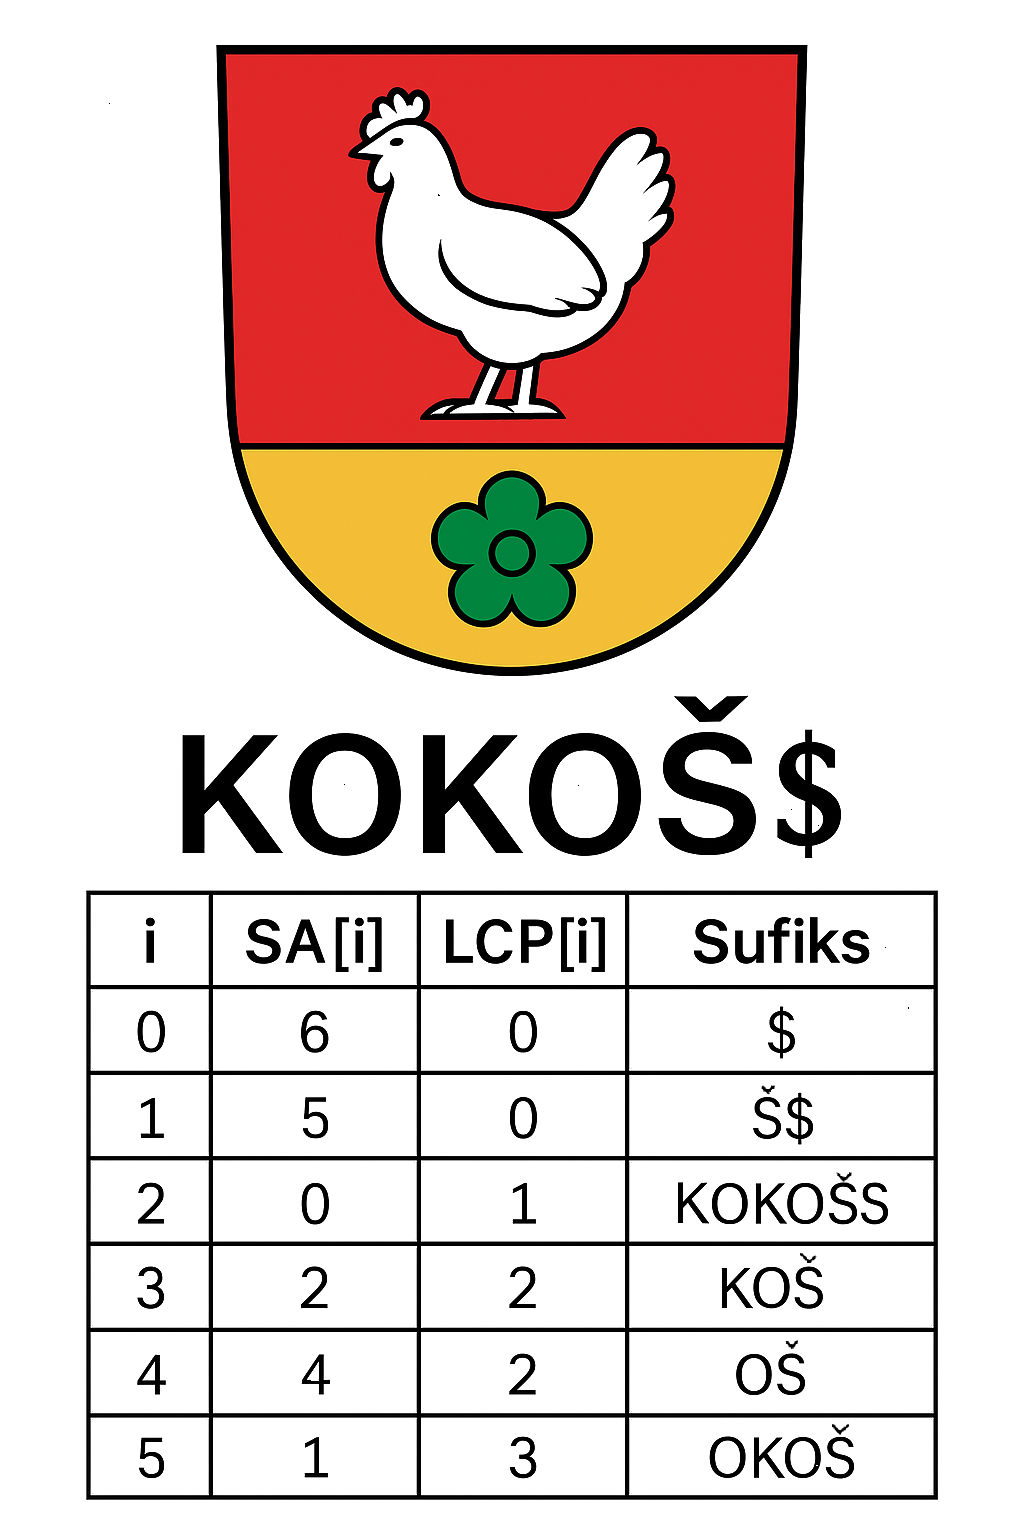
\includegraphics[width=.5\textwidth]{Slike/ChatGPTSA.png}
%        \caption{Primer priponskega polja nad besedo \enquote{KOKOŠ$\$$} kot si jo predstavlja ChatGPT.} 
%        \label{fig:ChatGPT}
%    \end{center}
%\end{figure}



%\section{NAJDALJŠA SKUPNA PREDPONA}\label{sec:LCP}
%\import{.}{PriponskoPolje/LCP}

\section{POIZVEDBE}\label{sec:SAPoizvedbe}
\import{.}{PriponskoPolje/Poizvedba}


\section{GRADNJA}\label{sec:SAIzgradnja}
\import{.}{PriponskoPolje/Izgradnja}

\section{SIMULACIJA OPERACIJ PRIPONSKEGA DREVESA}\label{sec:STsimulacija}
\import{.}{PriponskoPolje/SimulacijaDrevesa}